\chapter{Utilizzo del debugger}
È possibile avviare l'interfaccia di debug tramite l'apposita scheda \ref{fig:startDebug} (pin 1) e poi dopo aver selezionato la configurazione \codeword{launch nmd}  dal menù a tendina \ref{fig:startDebug} (pin 2)si avvia la sessione premendo il tasto di avvio collocato accanto allo stesso menù.  

\begin{figure}[H]
    \centering
    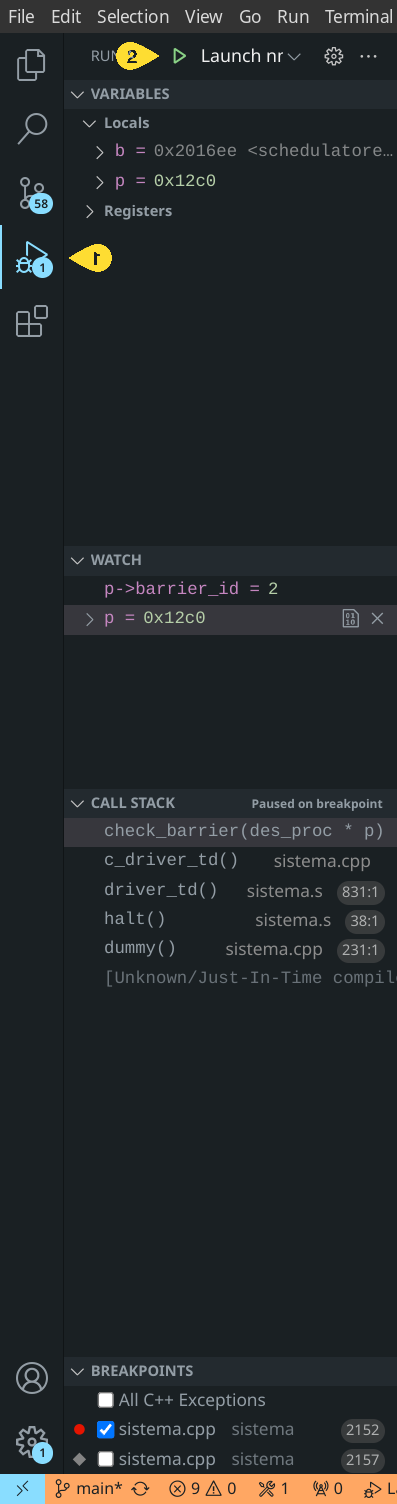
\includegraphics[height=0.3\pdfpageheight]{images/startDebug.png}
    \caption{Azioni per avviare il debug}
    \label{fig:startDebug}
\end{figure}

oppure premendo il tasto \codeword{F5} sulla tastiera.

L'interfaccia che ci viene presentata è la seguente 

\begin{figure}[H]
    \centering
    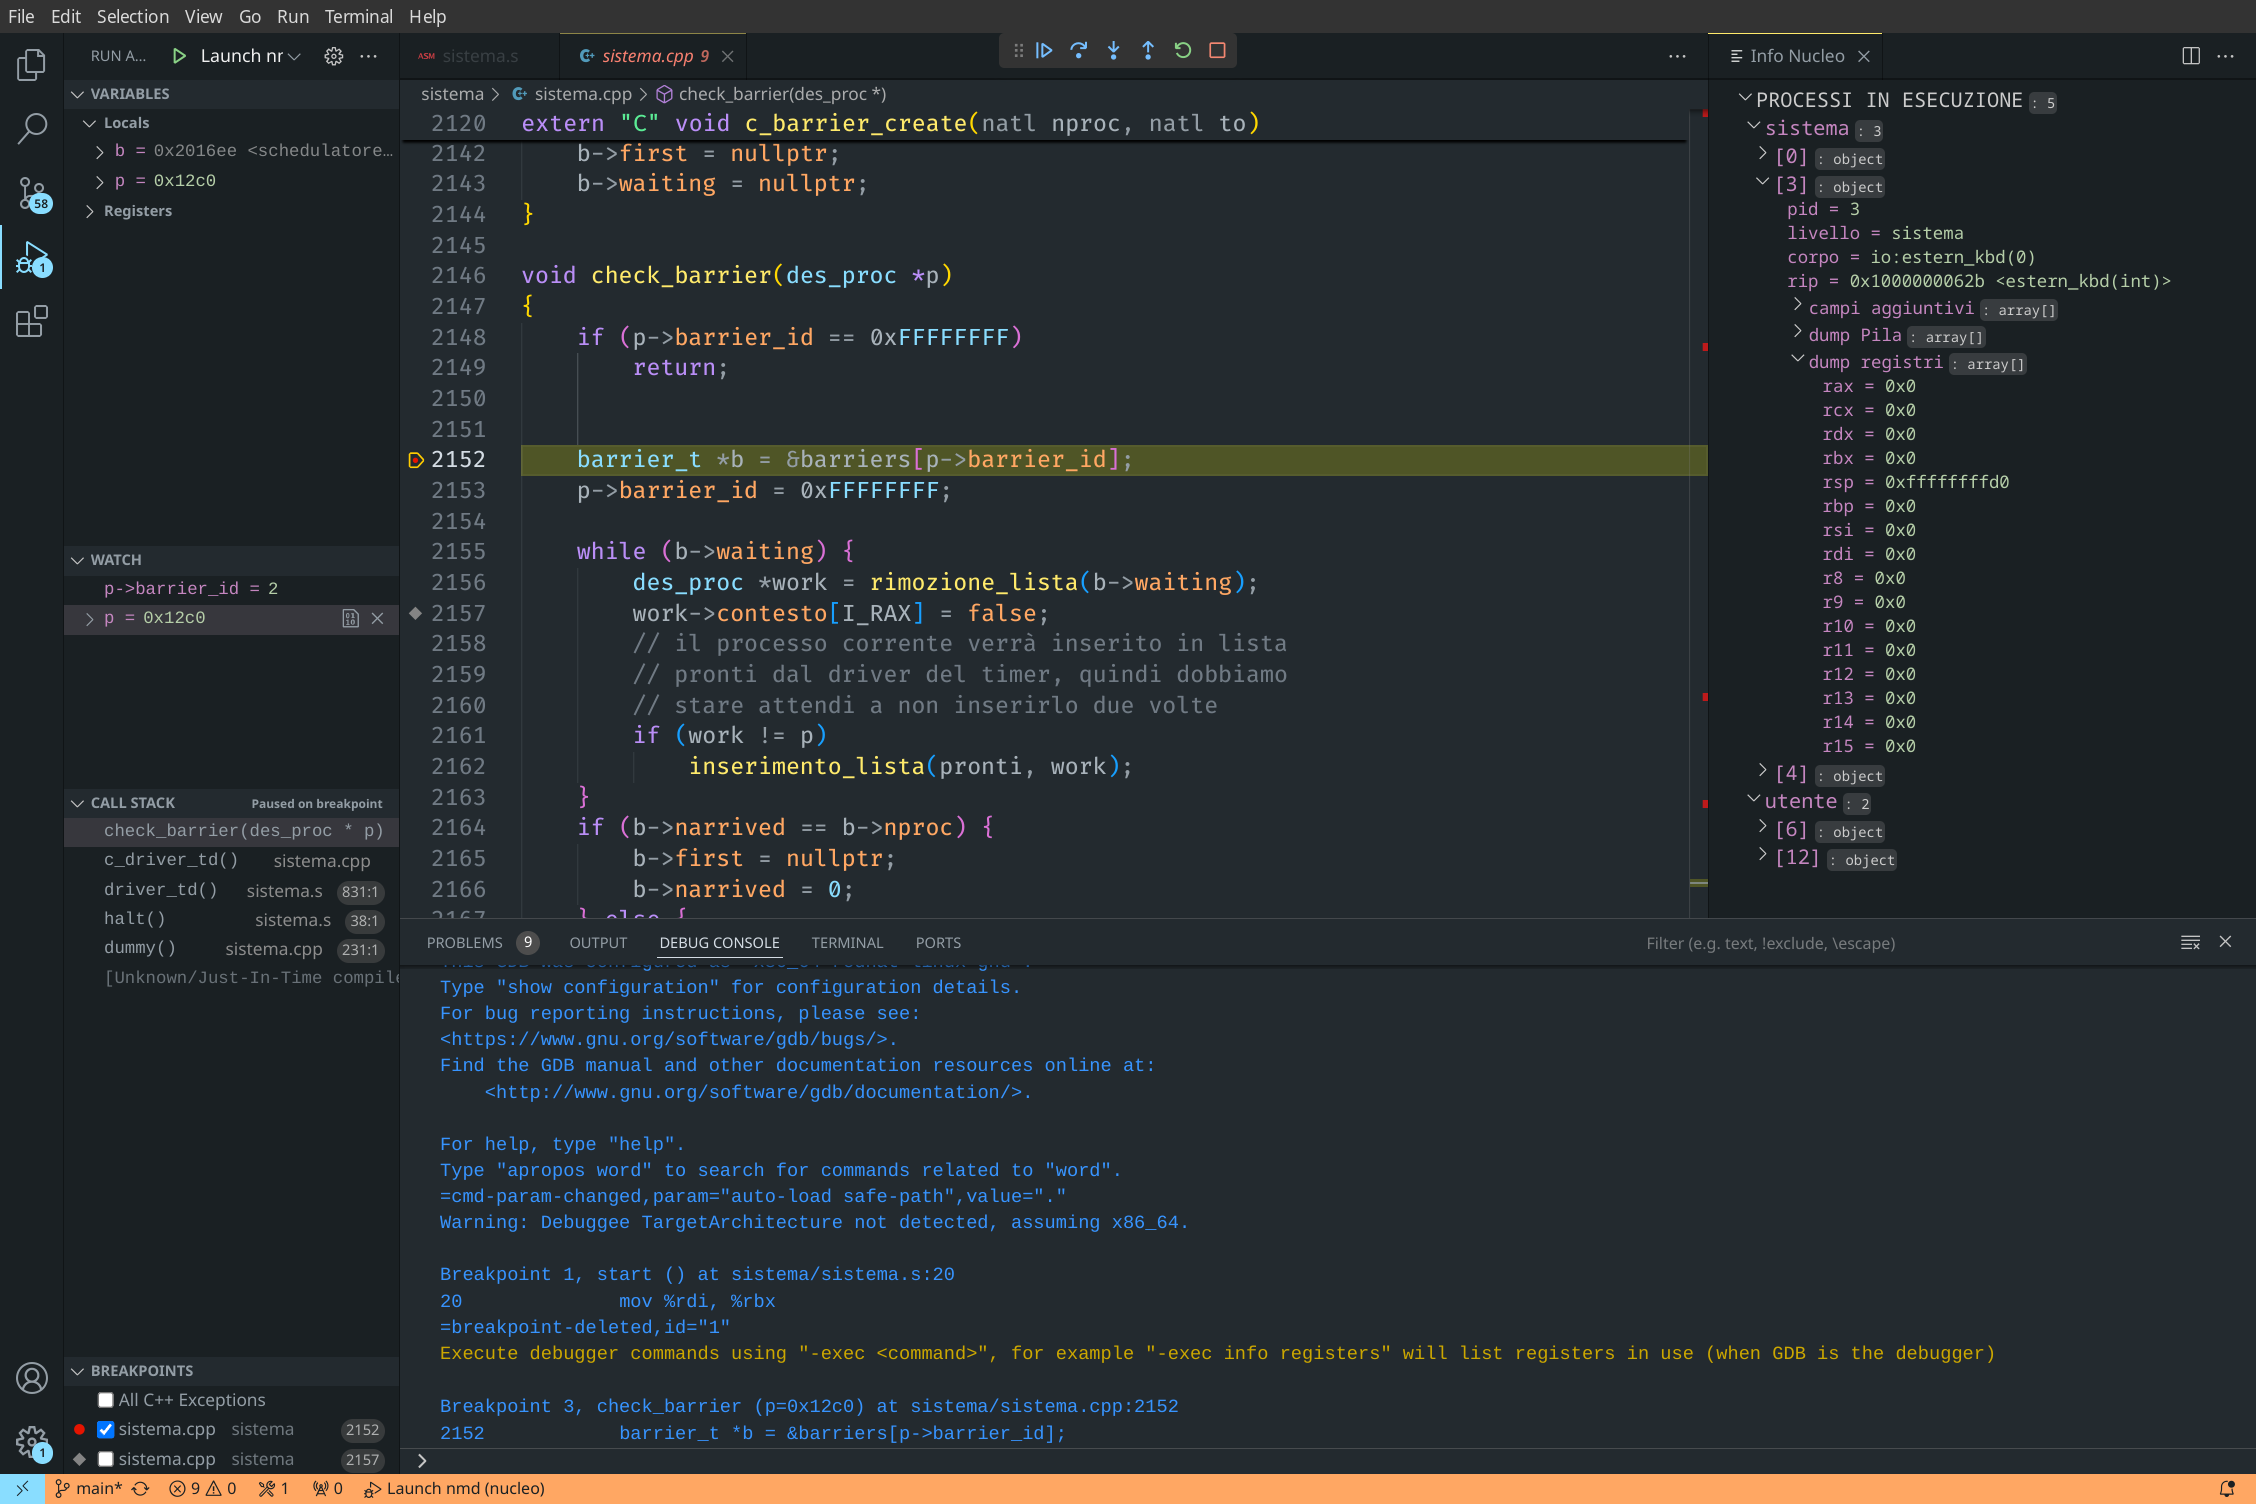
\includegraphics[width=\columnwidth]{images/fullDebug.png}
    \caption{Interfaccia di debug di  VSCode}
    \label{fig:debug screen}
\end{figure}

Analizziamo le varie finestre che ci vengono proposte.

\section{Breakpoint e Logpoint}
Nella vista del codice sorgente è possibile inserire un breakpoint premendo sul lato sinistro del numeri di rigainteressato, VSCode stesso si occuperà poi di comunicare al Debug Adapter la richiesta di inserimento del breakpoint.

\begin{figure}[H]
    \centering
    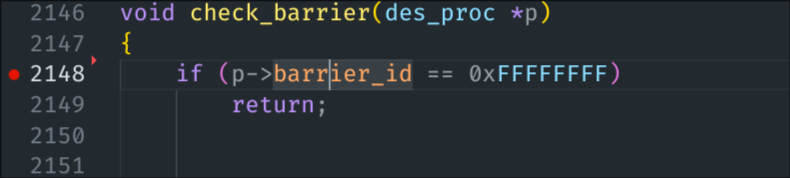
\includegraphics[width=0.7\columnwidth]{images/breakpoint_vscode.png}
    \caption{Esempio di un breakpoint in VSCode}
    \label{fig:breakpoint}
\end{figure}

Similarmente si può inserire un logpoint premendo con il tasto destro del mouse e selezionando la dicitura logpoint. All'interno del box di testo si possono aggiungere le variabili da osservare tramite \codeword{{{variable}}}

\begin{figure}[H]
    \centering
    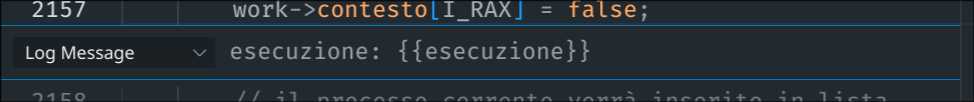
\includegraphics[width=0.7\columnwidth]{images/logpoint.png}
    \caption{Esempio di logpoint}
    \label{fig:logpoint}
\end{figure}

una volta ripresa l'esecuzione del codice possiamo vedere l'output nella console di debug.

\section{Azioni di debug}

VSCode mette a disposizione una barra di funzioni \ref*{fig:middleDebug}(pin 1) per permettere all'utente di ispezionare il codice tramite i comandi di step over, step in e step out. È possibile anche eseguire azioni come continue, stop e il riavvio della sessione di debug.  

\begin{figure}[H]
    \centering
    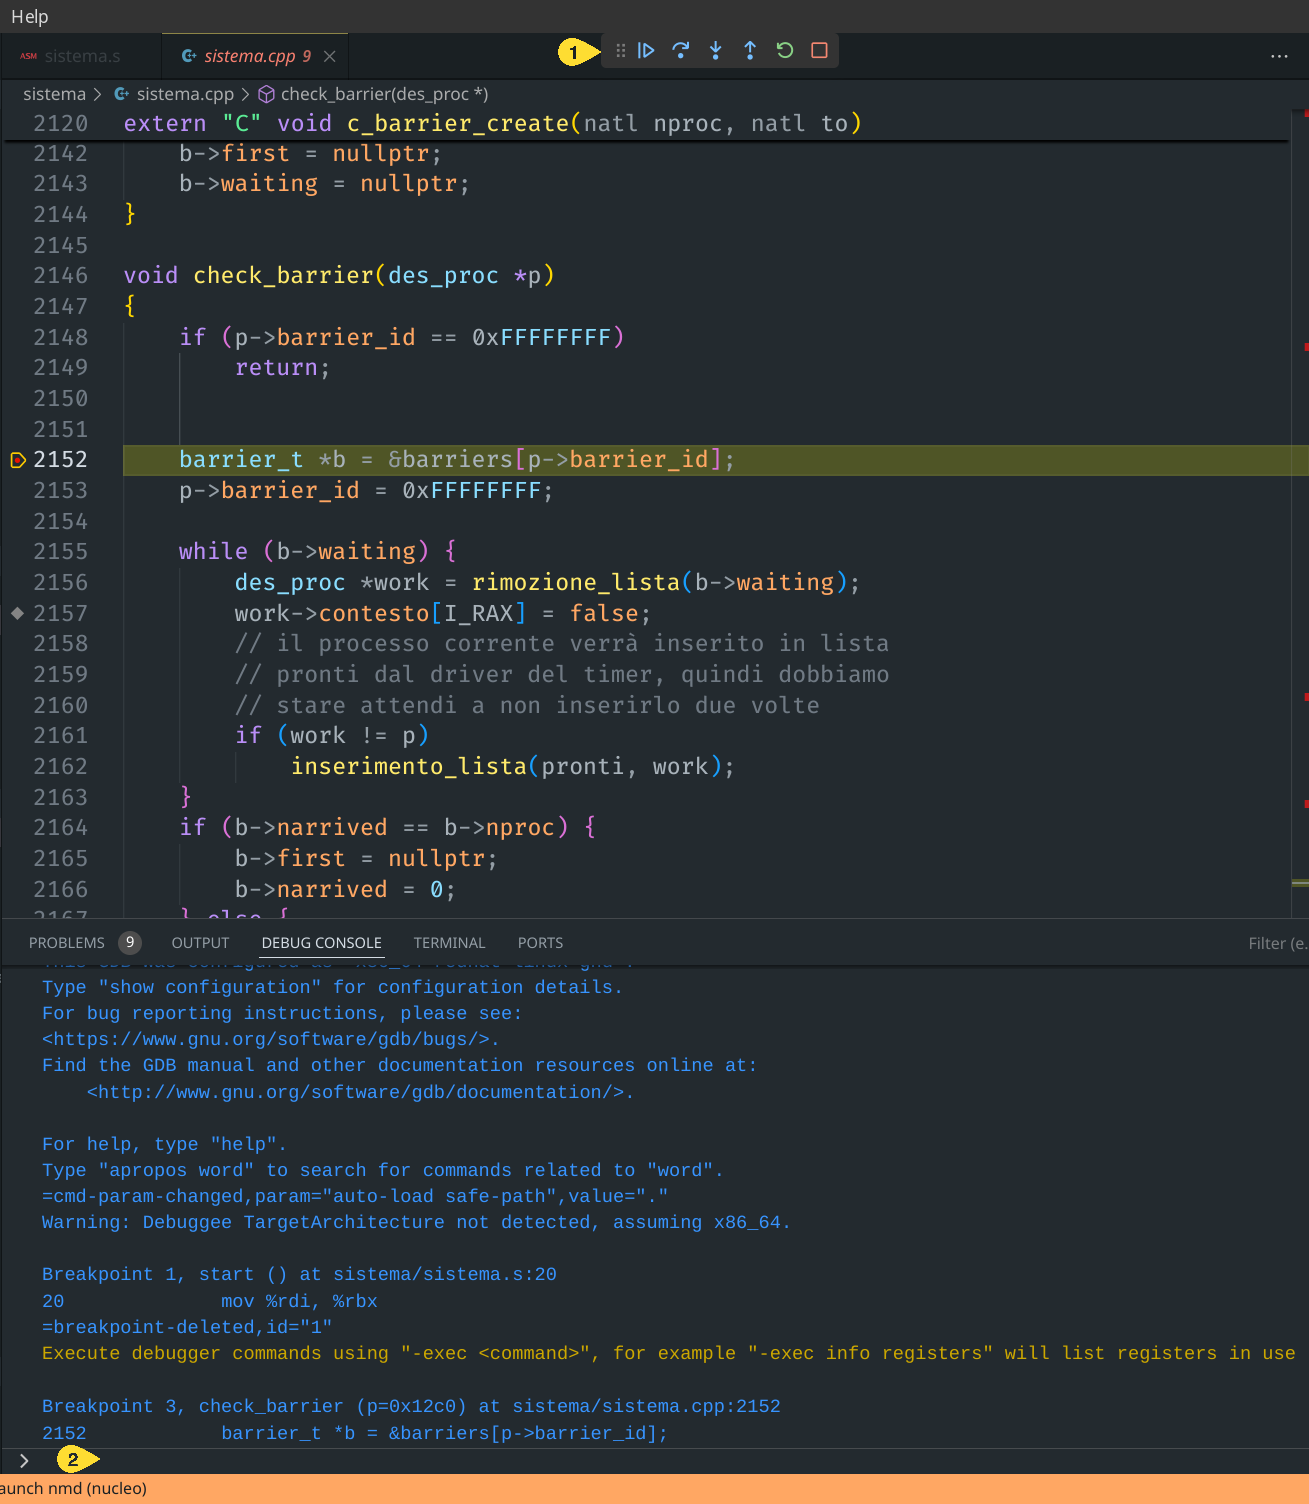
\includegraphics[width=0.8\columnwidth]{images/middle_debug.png}
    \caption{Azioni e linea di comando}
    \label{fig:middleDebug}
\end{figure}

Inoltre è possibile inviare comandi di GDB direttamente dalla linea di comando \ref*{fig:middleDebug}(pin 2) tramite il comando \codeword{-exec [GDB command]}.

\section{Pannello di sinistra}

Il pannello di sinistra permette di analizzare lo stato delle variabili locali \ref*{fig:leftDebug}(pin 2) e lo stato dei registri \ref*{fig:leftDebug}(pin 3).

\begin{figure}[H]
    \centering
    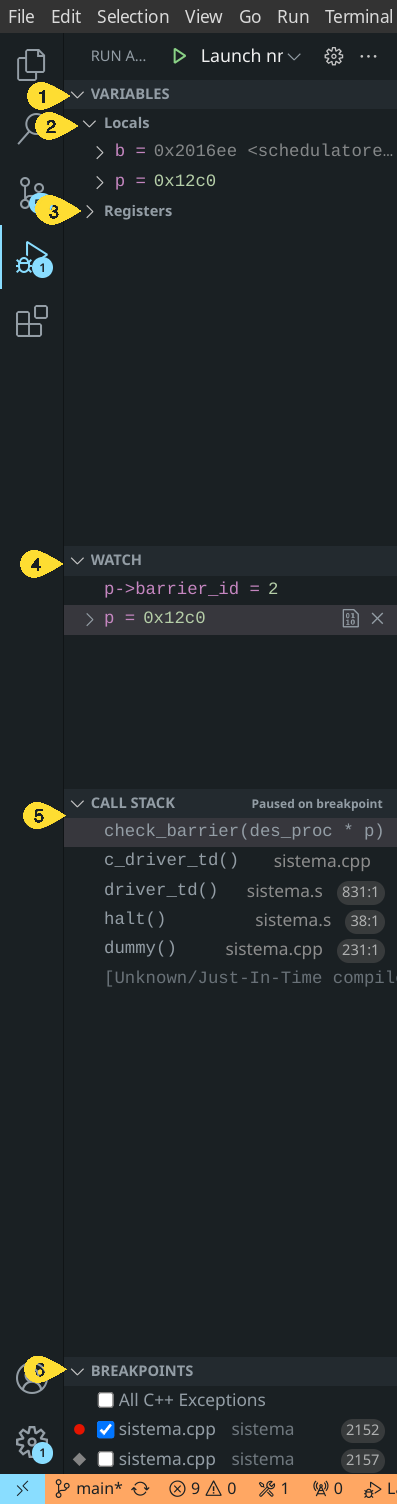
\includegraphics[height=0.4\pdfpageheight]{images/leftDebug.png}
    \caption{Azioni e linea di comando}
    \label{fig:leftDebug}
\end{figure}

\subsection*{Watch}
Nel pannello dedicato \ref*{fig:leftDebug}(pin 4) possiamo visualizzare le variabili messe sotto osservazione. L'aggiunta può avvenire tramite il pulsante "+" oppure selezionando con il cursore la variabile o l'espressione da analizzare e cliccando con il tasto destro dal menù a tendina selezionare "Add to watch" come mostrato in figura.

\begin{figure}[H]
    \centering
    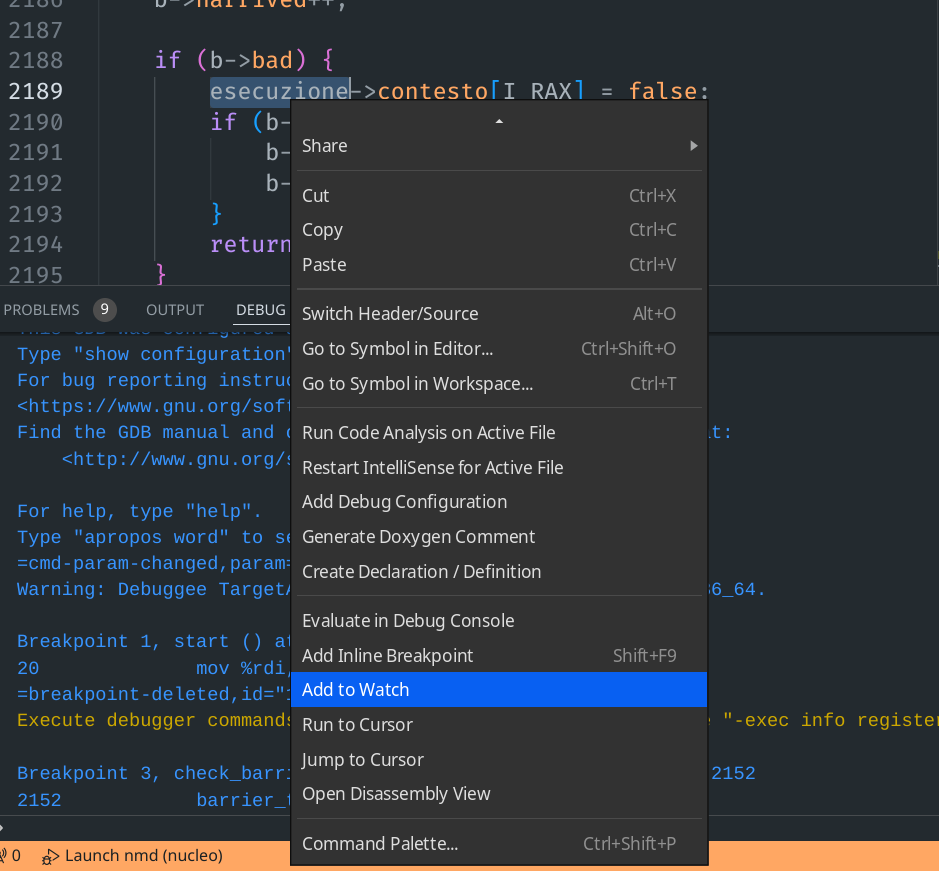
\includegraphics[width=0.8\columnwidth]{images/addWatch.png}
    \caption{Aggiunta al watch di una variabile}
    \label{fig:watchvariabili}
\end{figure}

\subsection*{Call stack e breakpoints}
È inoltre possibile visualizzare informazioni riguardanti il call stack \ref*{fig:leftDebug}(pin 5) e gestire i breakpoint presenti tramite il pannello dedicato \ref*{fig:leftDebug}(pin 6)

\section{Informazioni aggiuntive}

Sulla parte destra della finestra di debug troviamo la scheda dedicata alle informazioni aggiuntive del Nucleo. In questo caso
mostra solo i processi in esecuzione 

\begin{figure}[H]
    \centering
    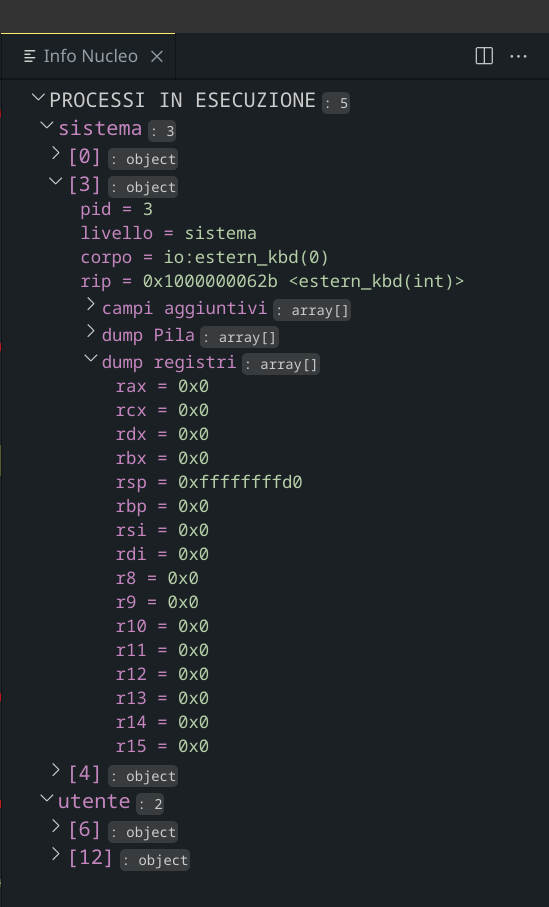
\includegraphics[height=0.3\pdfpageheight]{images/infoNucleo.png}
    \caption{Informazioni aggiuntive sul nucleo}
    \label{fig:infoNucleo}
\end{figure}

\subsection*{Processi in esecuzione}
Le informazioni relative ai processi vengono mostrate tramite una lista con elementi selezionabili. Ogni elemento della lista è formato da una rappresentazione tramite \codeword{chiave:valore} e un eventuale campo adiacente con eventuali informazioni sulla tipologia della variabile o oggetto. I processi sono stati divisi per convenienza tra processi di sistema e processi utente. 



